\section{Background}

\subsection{Strongly Connected Components}
\begin{frame}
	\frametitle{Serial Algorithms}
	\begin{itemize}
		\setlength\itemsep{1em}
		\item Tarjan's Algorithm
		\item Kosaraju's Algorithm
	\end{itemize}
\end{frame}

\begin{frame}
	\frametitle{Forward-Backword Algorithm}
	\begin{itemize}
		\setlength\itemsep{1em}
		\item Let $V$ denote the set of vertices in the graph,
			$E(V)$ the set of outgoing edges, and $E'(V)$ the set
			of incoming edges.
		\item Given the graph $G(V, E(V))$, a pivot vertex $u$ is selected.
		\item A BFS search is conducted starting from $u$ to determine all 
			vertex vertices. We get \textit{descendant} set $D$ on $G(V, E(V))$ 
			and \textit{predecessor} set $P$ on $G(V, E'(V))$.
		\item The SCC $S = D \cap P$ has the pivot $u$ in it.
		\item It can be recursively called on ($D \setminus S$), 
			$(P \setminus S)$, and $(V \setminus (P \cup D))$.
	\end{itemize}
\end{frame}

\begin{frame}
	\begin{figure}
		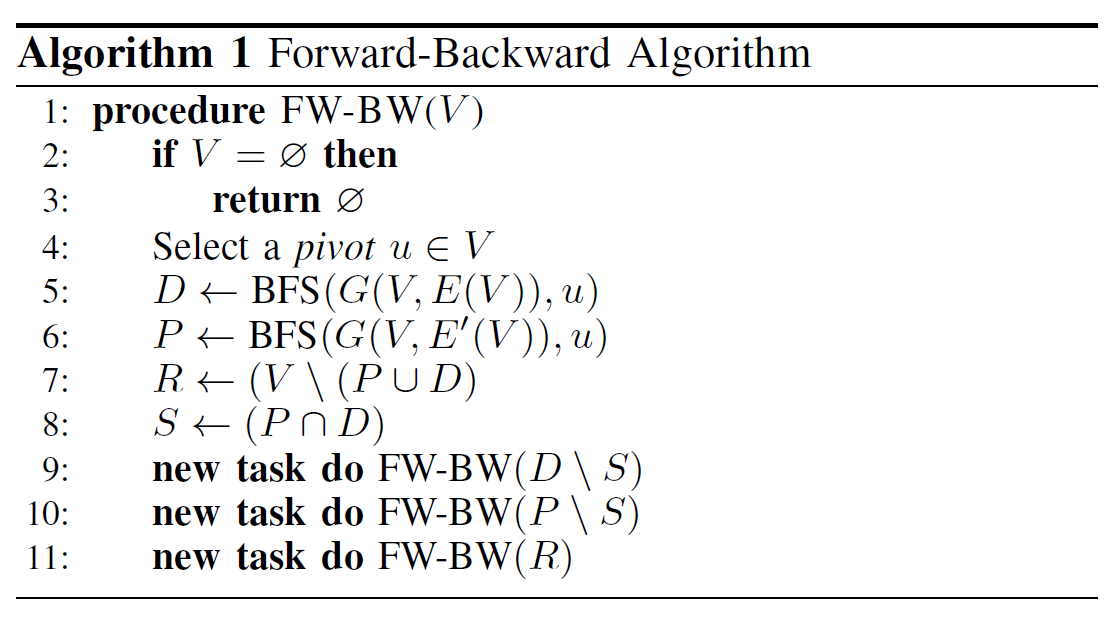
\includegraphics[scale=0.30]{figure/fig-FW-BW.png}
	\end{figure}
	\begin{itemize}
		\item For graphs with bounded constant vertex degree, 
			FW-BW is shown to perform $O(n \log n)$ expected case work.
	\end{itemize}
\end{frame}

\begin{frame}
	\frametitle{Coloring Algorithm}
	\begin{itemize}
		\setlength\itemsep{1em}
		\item This algorithm is similar to FW-BW in that it uses 
			forward and backward traversals.
		\item It uses multiple pivots in the forward phase and only looks at a 
			subset of edges for each pivot in the backward phase.
		\item In a graph with a very large SCC and high diameter, the color of
			the root vertex has to be propagated to all of the verties in the
			SCC, limiting the efficiency of the color propagation step.
	\end{itemize}
\end{frame}

\begin{frame}
	\begin{figure}
		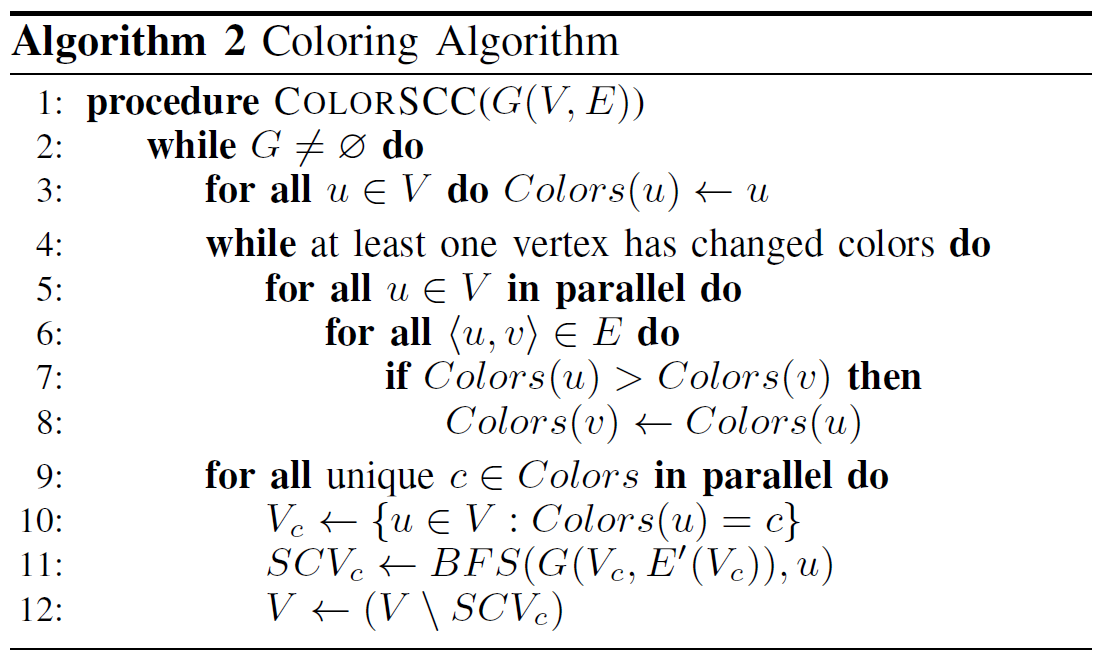
\includegraphics[scale=0.30]{figure/fig-Coloring.png}
	\end{figure}
\end{frame}

\subsection{Weakly Connected Components}
\begin{frame}
	\frametitle{Weakly Connected Components}
	There are two primary parallel methods:
	\begin{itemize}
		\setlength\itemsep{1em}
		\item Parallel BFS can be used for connected components. 
			We select new unvisted vertices as BFS roots until all vertices 
			have been visited and all connected components identified.
		\item We can use a coloring approach. Once the colors reach 
			a stable point, all vertices contained in each discrete 
			component will have the same color. \#propagation iterations 
			is bounded by $O(\log n)$.
	\end{itemize}
\end{frame}

\subsection{Biconnected Components}
\begin{frame}
	\frametitle{Biconnected Components}
	\begin{itemize}
		\setlength\itemsep{1em}
		\item The Hopcroft-Tarjan algorithm is the optimal linear-time sequential algorithm, which is based on DFS.
		\item The Tarjan-Vishkin parallel algorithm voids DFS.
	\end{itemize}
\end{frame}

